\documentclass[tikz,border=8pt]{standalone}

\usepackage[T1]{fontenc}
\usepackage[utf8]{inputenc}
\usepackage{lmodern}
\usepackage{tikz}
\usetikzlibrary{arrows.meta, positioning}

\begin{document}
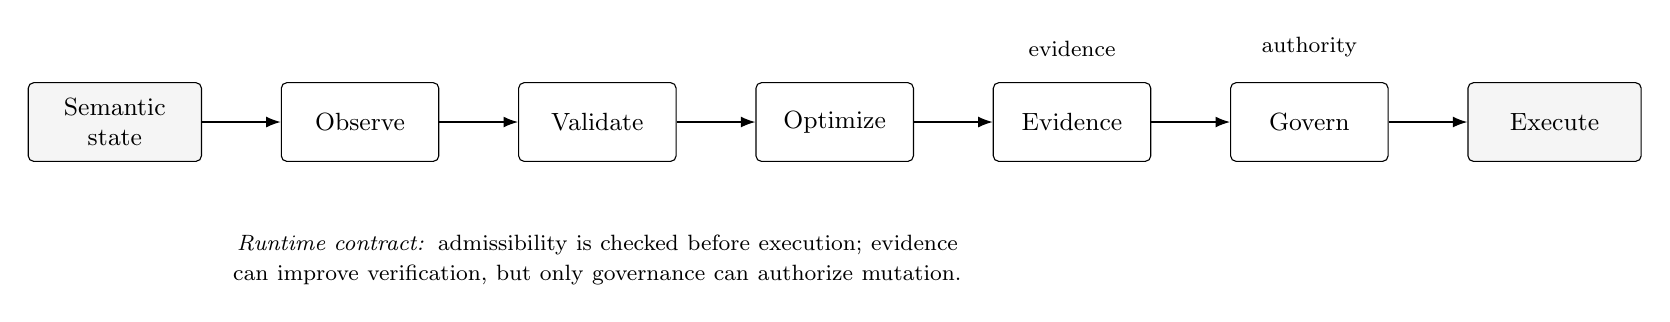
\begin{tikzpicture}[
  font=\small,
  node distance=7mm and 10mm,
  box/.style={draw, rounded corners=2pt, align=center, minimum width=20mm, minimum height=10mm, fill=white, line width=0.4pt},
  muted/.style={draw, rounded corners=2pt, align=center, minimum width=22mm, minimum height=10mm, fill=gray!8, line width=0.4pt},
  arrow/.style={-Latex, line width=0.5pt}
]
  \node[muted] (state) {Semantic\\state};
  \node[box, right=of state] (obs) {Observe};
  \node[box, right=of obs] (val) {Validate};
  \node[box, right=of val] (opt) {Optimize};
  \node[box, right=of opt] (evi) {Evidence};
  \node[box, right=of evi] (gov) {Govern};
  \node[muted, right=of gov] (exec) {Execute};

  \draw[arrow] (state) -- (obs);
  \draw[arrow] (obs) -- (val);
  \draw[arrow] (val) -- (opt);
  \draw[arrow] (opt) -- (evi);
  \draw[arrow] (evi) -- (gov);
  \draw[arrow] (gov) -- (exec);

  \node[draw=none, below=8mm of val, align=center, text width=0.78\linewidth] (contract)
  {\footnotesize \textit{Runtime contract:} admissibility is checked before execution; evidence can improve verification, but only governance can authorize mutation.};
\node[draw=none, above=2mm of evi, align=center, text width=0.18\linewidth] (evidence_label)
  {\footnotesize evidence};
\node[draw=none, above=2mm of gov, align=center, text width=0.18\linewidth] (authority_label)
  {\footnotesize authority};
\end{tikzpicture}
\end{document}
